\chapter{Modelling and Control}

\section{The mechanics of a quadrotor}
This section will explain how the quadrotor moves in each direction as well as how it is able to rotate around each of the body-fixed axes.
\lipsum[1-10]
\section{Deriving the equations of motion}
The Newton-Euler derivation of the equation of motion.

\begin{equation}
    m \ddot{\textbf{r}} = \begin{bmatrix}
        0 \\ 0 \\ -mg
    \end{bmatrix}
    + R \begin{bmatrix}
    0 \\ 0 \\ F_1+F_2+F_3+F_4
    \end{bmatrix}
\end{equation}

\begin{equation}
    I \begin{bmatrix} \dot{p} \\ \dot{q} \\ \dot{r} \end{bmatrix} = \begin{bmatrix} L(F_2-F_4) \\ L(F_3-F_1) \\ M_1-M_2+M_3-M_4 \end{bmatrix} - \begin{bmatrix} p \\ q \\ r \end{bmatrix} \times I \begin{bmatrix} p \\ q \\ r \end{bmatrix}
\end{equation}

\lipsum[1-10]
\begin{figure}
    \centering
    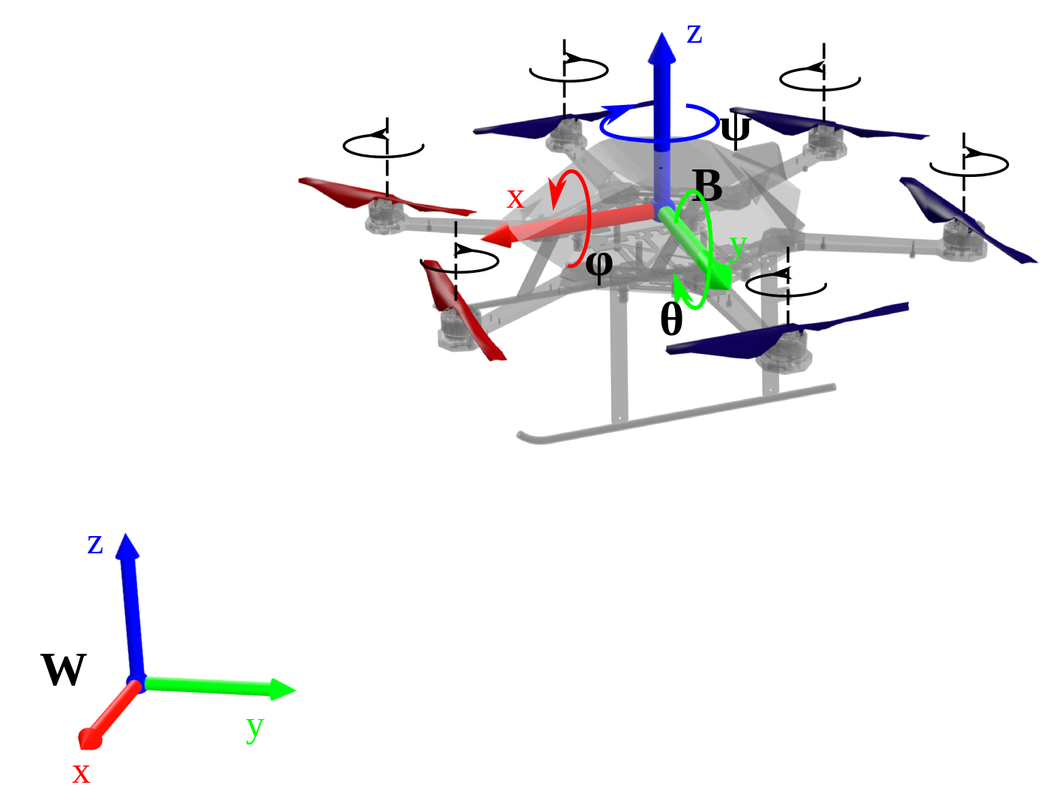
\includegraphics[width=\textwidth]{images/4464460_orig.png}
    \caption{The world and body-fixed frames}
    \label{fig:frames}
\end{figure}